\section{Results and Discussion}
\label{sec:results}

Experiments~A--C verify the individual subsystems against independent
references, D and E compare design choices within the estimator and the
controller, and F closes the loop and characterises the operating envelope.
Every number below is produced by the scripts named in Sec.~\ref{sec:method}
and is reproducible from the stated seeds.

\subsection{Dynamics Validation}
\label{sec:res_dynamics}

The numerical propagator was validated against the analytical HCW
state-transition solution over three orbital periods, using DOP853 with
relative and absolute tolerances of $10^{-12}$ and $10^{-14}$. The maximum
position discrepancy was $4.55\times10^{-10}$~m and the maximum velocity
discrepancy $5.38\times10^{-13}$~m/s.
Sweeping the tolerance reduces the maximum position error monotonically from
$4.50\times10^{-4}$~m at $(10^{-6},10^{-8})$ to $4.73\times10^{-11}$~m at
$(10^{-13},10^{-15})$: the integrator is converging, not merely reporting
small residuals. Two significant digits are quoted because the adaptive DOP853 step sequence
depends on the SciPy release, across whose tested versions the result moves by
a few per cent. The numerical error is sub-nanometre, nine orders of magnitude below the
metre-level separations of interest and eight below the centimetre-level pose
errors of Sec.~\ref{sec:res_pose}, and is therefore not a contributor to any
subsequent result.


\subsection{Vision-Based Pose Estimation}
\label{sec:res_pose}

Table~\ref{tab:pose_noise} and Fig.~\ref{fig:pose_noise} report pose
sensitivity to image-plane noise at a fixed 20~m range and attitude.

\begin{table}[!tb]
\caption{Pose error against keypoint noise. 200 trials per level, 15
keypoints, 20~m range. RMSE over successful solves.}
\label{tab:pose_noise}
\centering
\begin{tabular}{lllllr}
\hline
$\sigma_{px}$ & \multicolumn{2}{c}{EPnP} & \multicolumn{2}{c}{EPnP + LM} & solved \\
{}[px] & $t$ [cm] & $\theta$ [$^\circ$] & $t$ [cm] & $\theta$ [$^\circ$] & \\
\hline
0.10 & 0.400  & 0.056 & 0.362  & 0.048 & 200/200 \\
0.25 & 1.142  & 0.143 & 0.982  & 0.128 & 200/200 \\
0.50 & 2.056  & 0.275 & 1.732  & 0.249 & 200/200 \\
1.00 & 4.384  & 0.567 & 3.986  & 0.511 & 200/200 \\
1.50 & 6.302  & 0.865 & 5.695  & 0.787 & 200/200 \\
2.00 & 7.836  & 1.095 & 7.065  & 1.025 & 200/200 \\
3.00 & 13.766 & 1.696 & 11.492 & 1.533 & 200/200 \\
5.00 & 23.463 & 2.885 & 20.293 & 2.553 & 199/200 \\
\hline
\end{tabular}
\end{table}

Both errors grow essentially linearly with $\sigma_{px}$, as expected with the
geometry fixed and the noise small enough for the linearisation about the
true pose to hold. At 20~m and $f = 800$~px a 1~px displacement subtends
2.5~cm, consistent with the observed 4.38~cm translation RMSE at
$\sigma_{px} = 1$~px given 15 keypoints spanning a $372 \times 112$~px image
patch.

Levenberg--Marquardt refinement reduces translation error by 9--14\% and
attitude error by 10--14\% over the range tested. We report this modest gain
as such because a much larger apparent benefit is easy to obtain
accidentally: the closed-form stage of EPnP is accurate only if the
control-point coefficients $\beta_k$ are themselves refined against the
inter-control-point distance constraints (Sec.~\ref{sec:epnp_gn}) rather than
read directly off the linearised system in the products $\beta_k\beta_l$.
Omitting that internal refinement degrades raw EPnP by roughly a factor of
four, which then makes the LM stage appear to deliver a large gain. With the
reference algorithm implemented in full, most of the achievable accuracy is
present before LM runs.

Three cross-checks support the implementation: our EPnP agrees with the
OpenCV \texttt{SOLVEPNP\_EPNP} reference to within a factor of 1.2 in rotation
error at $\sigma_{px} = 1$~px; the refined solver matches
\texttt{cv2.solvePnPRefineLM} to four decimal places at every noise level; and
exactly coplanar keypoint subsets are solved to $0.0000^\circ$, a case the
OpenCV EPnP implementation does not handle and one arising in approximately
3\% of random six-point samples from this target's keypoint set.

\begin{figure}[!tb]
    \centering
    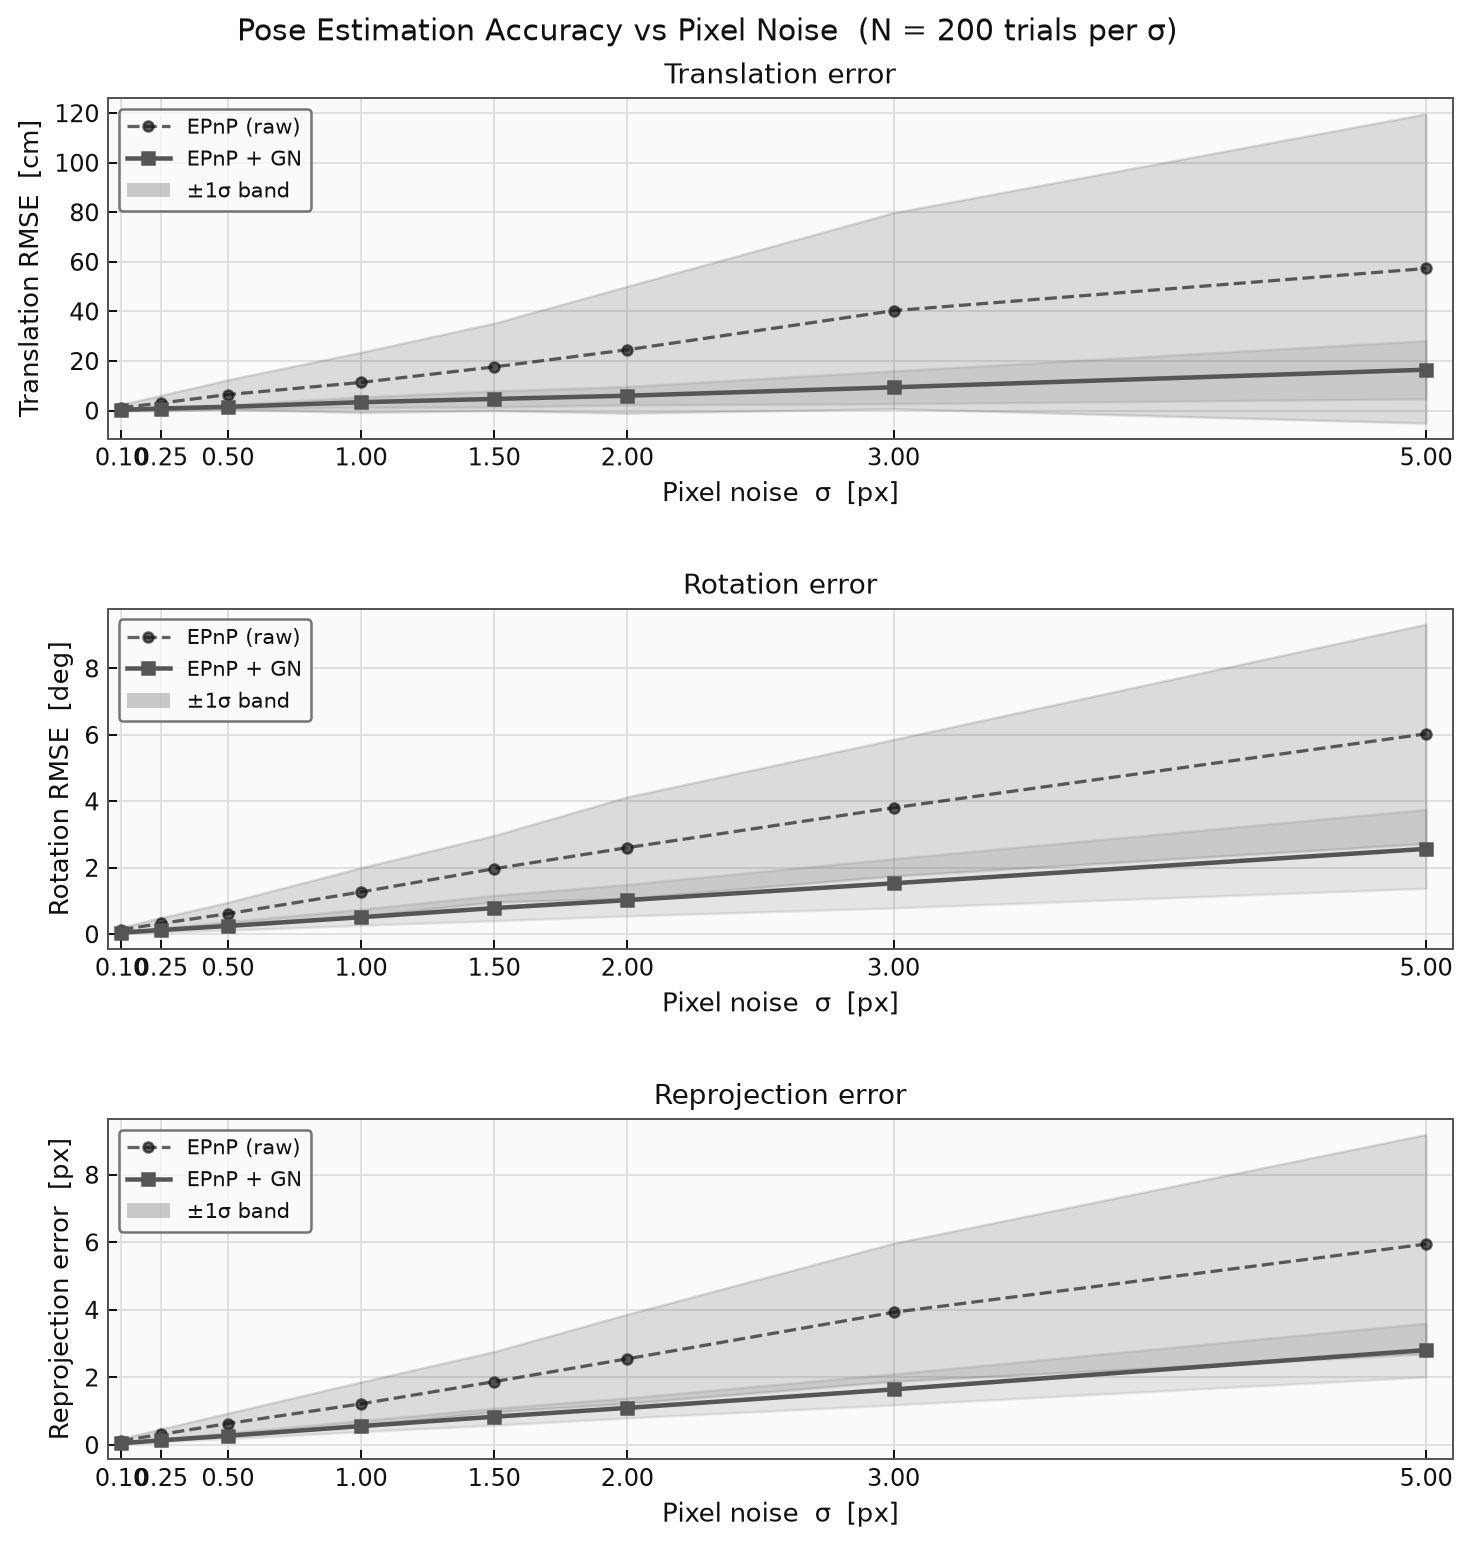
\includegraphics[width=0.86\columnwidth]
    {figures/expB_fig2_pose_vs_noise.png}
    \caption{Pose error against keypoint noise for raw EPnP and after
    Levenberg--Marquardt refinement. 200 trials per level.}
    \label{fig:pose_noise}
\end{figure}

\subsection{Robustness to Correspondence Outliers}
\label{sec:res_ransac}

Table~\ref{tab:ransac} reports the effect of replacing a fraction $f_{out}$ of
the 15 keypoints by uniformly distributed image points, with inlier noise held
at $\sigma_{px} = 1$~px.

\begin{table}[!tb]
\caption{Outlier robustness. 200 trials per level. Errors are RMSE over
successful trials; a dash indicates too few successes to report.}
\label{tab:ransac}
\centering
\begin{tabular}{lrllrll}
\hline
$f_{out}$ & \multicolumn{3}{c}{EPnP alone} & \multicolumn{3}{c}{RANSAC--EPnP} \\
& fail & $t$ [cm] & $\theta$ [$^\circ$] & fail & $t$ [cm] & $\theta$ [$^\circ$] \\
\hline
0\%  & 0\%   & 4.275  & 0.652 & 0\% & 5.175 & 0.854 \\
5\%  & 99\%  & 14.925 & 0.792 & 0\% & 5.364 & 0.842 \\
10\% & 100\% & --     & --    & 0\% & 5.615 & 0.927 \\
20\% & 100\% & --     & --    & 0\% & 6.363 & 0.917 \\
30\% & 100\% & --     & --    & 0\% & 6.074 & 1.037 \\
\hline
\end{tabular}
\end{table}

A single gross outlier destroys the least-squares solution: at
$f_{out} = 5\%$, fewer than one outlier per frame on average, bare EPnP fails
in 99\% of trials. Outlier rejection is not a refinement but a precondition
for applying a PnP solver to real correspondences. RANSAC--EPnP fails in no
trial up to $f_{out} = 30\%$ and degrades only mildly --- 5.18 to 6.07~cm in
translation, 0.854 to 1.037$^\circ$ in attitude --- growth consistent with the
reduced number of true inliers available to the final refit rather than with
any breakdown of the consensus search.

At $f_{out} = 0\%$ RANSAC is slightly \emph{worse} than bare EPnP (5.18~cm
against 4.275~cm). This is expected rather than a defect: the 2~px inlier gate
discards a few legitimate but noisy points, so the final refit uses less data.
Robustness carries a price, and disabling outlier rejection is reasonable when
correspondences are known to be clean.

\begin{figure}[!tb]
    \centering
    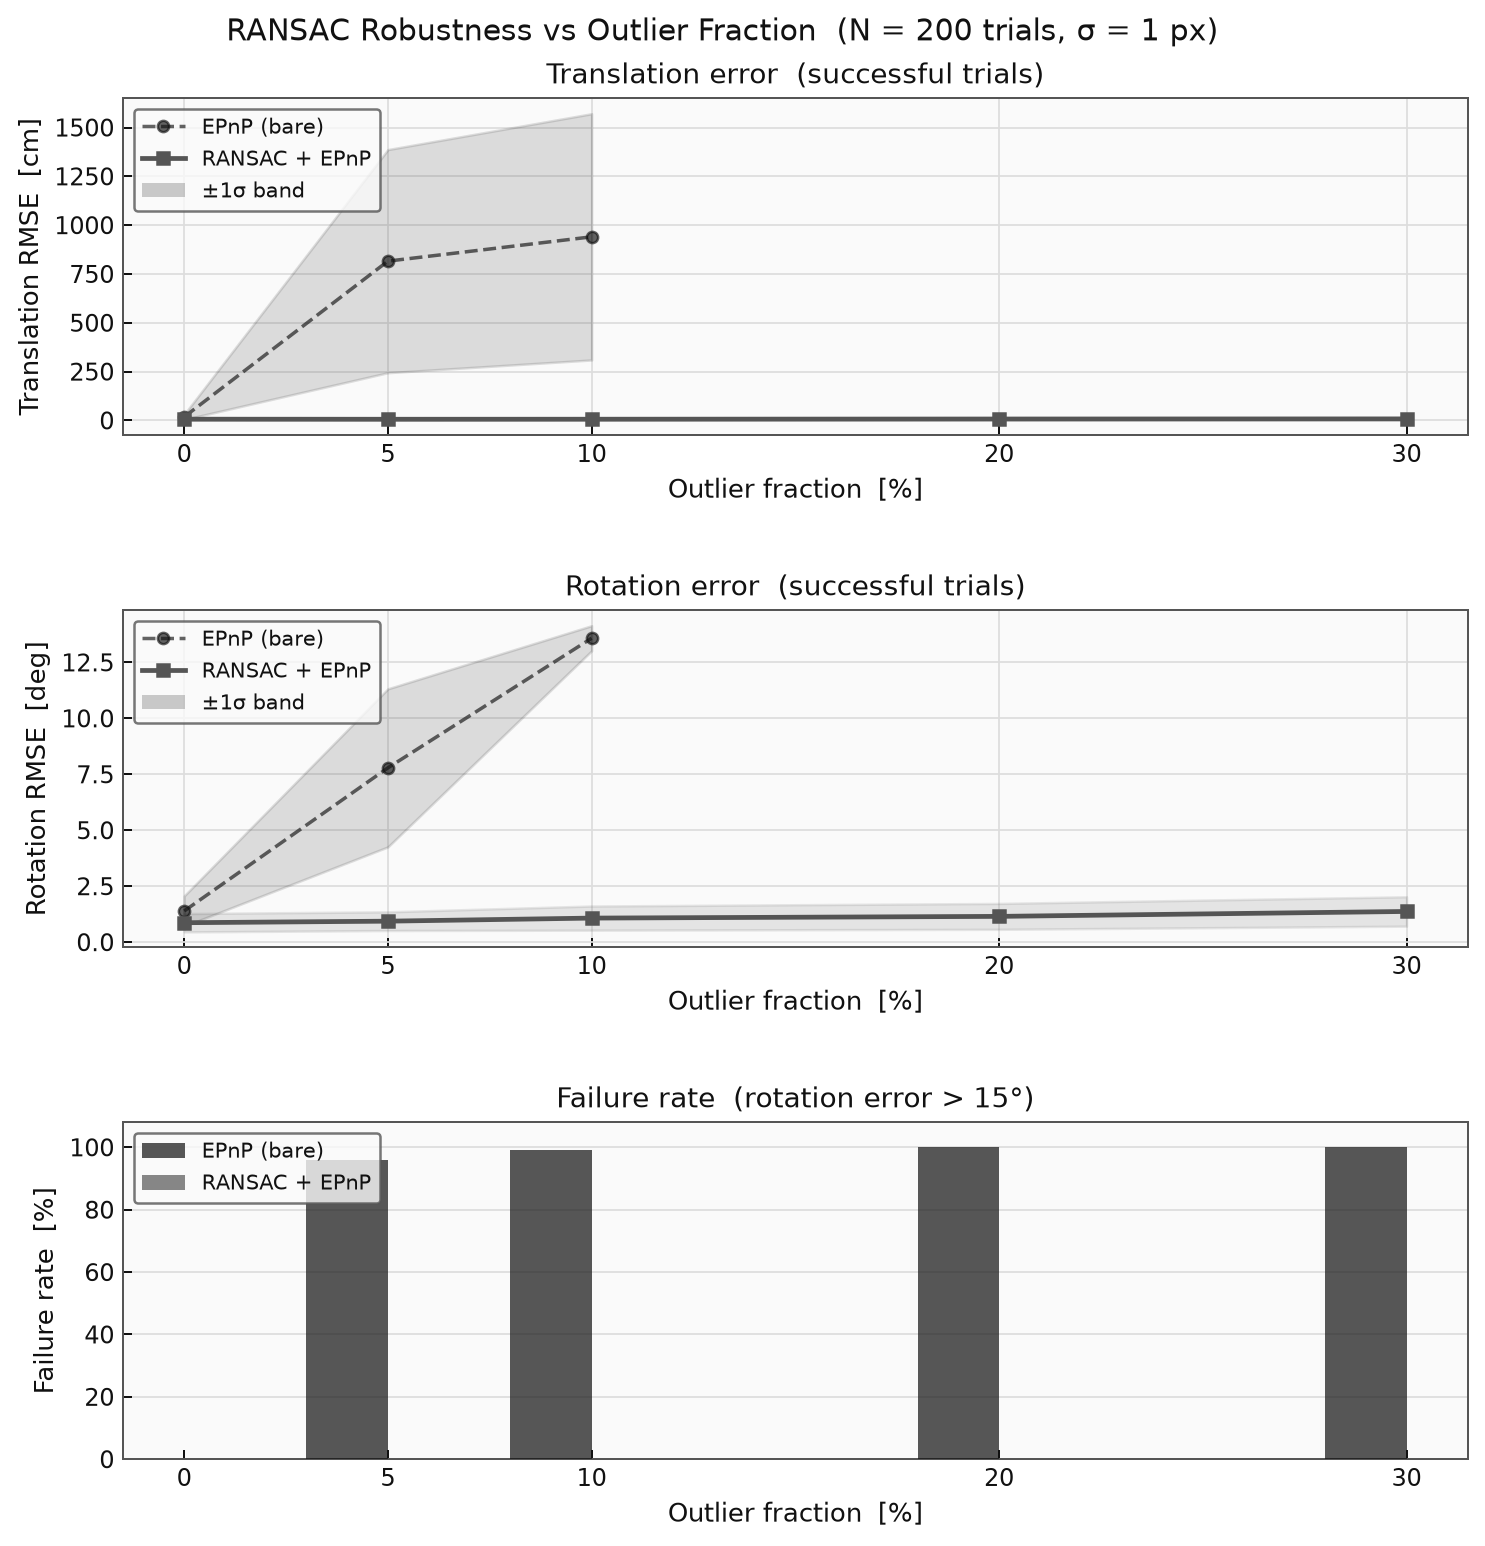
\includegraphics[width=0.86\columnwidth]
    {figures/expC_fig3_ransac_robustness.png}
    \caption{Pose error and failure rate against outlier fraction, for EPnP
    alone and for RANSAC--EPnP. 200 trials per level.}
    \label{fig:ransac_robustness}
\end{figure}

\subsection{Filter Comparison and Consistency}
\label{sec:res_filter}

Experiment~D isolates the estimator: both filters receive an identical
sequence of direct pose measurements over 300 steps, from an initial position
offset of 3.9~m and an initial attitude error of $17^\circ$, with the
perception chain replaced by an equivalent noise model so that filter
behaviour is not confounded with pose-solver failures.

\begin{table}[!tb]
\caption{Multiplicative EKF against UKF on identical measurements. 300 steps,
$\Delta t = 10$~s, seed 42.}
\label{tab:filters}
\centering
\begin{tabular}{lrr}
\hline
Metric & MEKF & UKF \\
\hline
Position RMSE [m]             & 0.5997  & 0.5997 \\
Attitude RMSE [$^\circ$]      & 1.2518  & 1.2802 \\
Velocity RMSE [m/s]           & 0.0226  & 0.0226 \\
Max position error [m]        & 1.5343  & 1.5343 \\
Max attitude error [$^\circ$] & 7.2282  & 7.7671 \\
Measurements accepted         & 300/300 & 300/300 \\
Wall-clock time [s]           & 1.602   & 1.662 \\
\hline
\end{tabular}
\end{table}

The two filters are indistinguishable in translation for a structural rather
than an empirical reason: HCW relative translation is exactly linear, so the
unscented transform and the analytic Jacobian describe the same map and must
agree to machine precision whatever the sigma-point spread. Any difference can
appear only through the attitude and rate block, and there the UKF is
marginally worse, and marginally \emph{slower} --- 1.662~s against 1.602~s,
3.7\% --- as expected of 25 sigma points per step against a single analytic
Jacobian propagation. We therefore find no advantage to the UKF for this
problem and use the MEKF throughout the closed-loop study. Two caveats: the
sigma-point spread parameter must be $O(0.1\text{--}1)$, since with the
frequently quoted $\alpha = 10^{-3}$ and $n_x = 12$ one obtains
$n_x + \lambda = 1.2\times10^{-5}$, a spread of $0.0035\sigma$ and a centre
weight of $-10^{6}$, at which point the unscented transform has collapsed onto
a finite-difference linearisation and an ``EKF versus UKF'' comparison
compares a filter with itself; and these timings are on unpinned consumer
hardware, so the 3.7\% gap should be read as ``no meaningful difference'', not
as a measurement.

Filter consistency is assessed through the normalised innovation squared,
\begin{equation}
\mathrm{NIS}_k = \boldsymbol{\nu}_k^{\top}\mathbf{S}_k^{-1}\boldsymbol{\nu}_k,
\label{eq:nis}
\end{equation}
which for a consistent filter is $\chi^2$ distributed with $n_z = 6$ degrees
of freedom. Over 3600 updates (12 seeds $\times$ 300 steps) the sample mean is
$\bar{\mathrm{NIS}} = 6.044$, against a 95\% confidence interval on the mean of
$[5.887,\,6.113]$ obtained from $n_z \pm 1.96\sqrt{2 n_z / N}$ using
$\mathrm{Var}[\chi^2_k] = 2k$; the fraction of updates exceeding
$\chi^2_{6,0.99} = 16.81$ is 0.97\%, against a nominal 1\%. The filter is
therefore consistent: its reported covariance matches the errors it actually
makes, and the Mahalanobis gate rejects at the designed rate.

This is a stronger statement than a small RMSE, and it rests on three
modelling choices that are easy to get wrong. The attitude residual must be
formed multiplicatively on $SO(3)$ (Sec.~\ref{sec:mekf_residual}); the process
noise must be acceleration-driven with the position--velocity cross terms
retained (Sec.~\ref{sec:process_noise}); and the truth must carry a
disturbance that the filter's $\mathbf{Q}$ actually describes. Substituting a
global rotation-vector residual yields
$\bar{\mathrm{NIS}} = 6.82$, an over-confident filter; removing the truth
disturbance yields 5.77, a conservative one.


\subsection{Guidance: LQR and MPC}
\label{sec:res_control}

Experiment~E compares the infinite-horizon LQR with the receding-horizon MPC
on a 50~m along-track approach, sharing weights, sample time and thrust limit,
with the LQR solution as the MPC terminal cost and the corridor disabled so
that thrust saturation is the only active constraint.


MPC reaches the same terminal accuracy for 5.00~m/s against 16.83~m/s, a 70\%
reduction in propellant. The mechanism must be stated precisely, because the
comparison is easy to over-read. With shared weights and the LQR terminal
cost, an MPC whose constraints are inactive reproduces the infinite-horizon
LQR exactly --- verified here to $4.8\times10^{-7}$. The entire difference is
therefore constraint handling, not prediction: the LQR gain demands
1.77~m/s$^2$ at the initial condition, seventeen times the actuator limit, and
is then clipped per axis, whereas MPC distributes the available authority over
its horizon. The honest framing is \emph{MPC against a saturated LQR}, and the
result is a statement about anti-windup; a constrained-LQR or
reference-governor baseline would narrow the gap and is the appropriate
comparison for future work.

The measured 0.57~ms per step reflects an active-set shortcut: the
corridor-constrained problem is solved only when the corridor is violated at
the box-constrained optimum. With the corridor active throughout, the per-step
cost rises by two orders of magnitude and is dominated by a few hard early
steps, for which a median and 95th percentile are the appropriate statistics.

\begin{figure}[!tb]
    \centering
    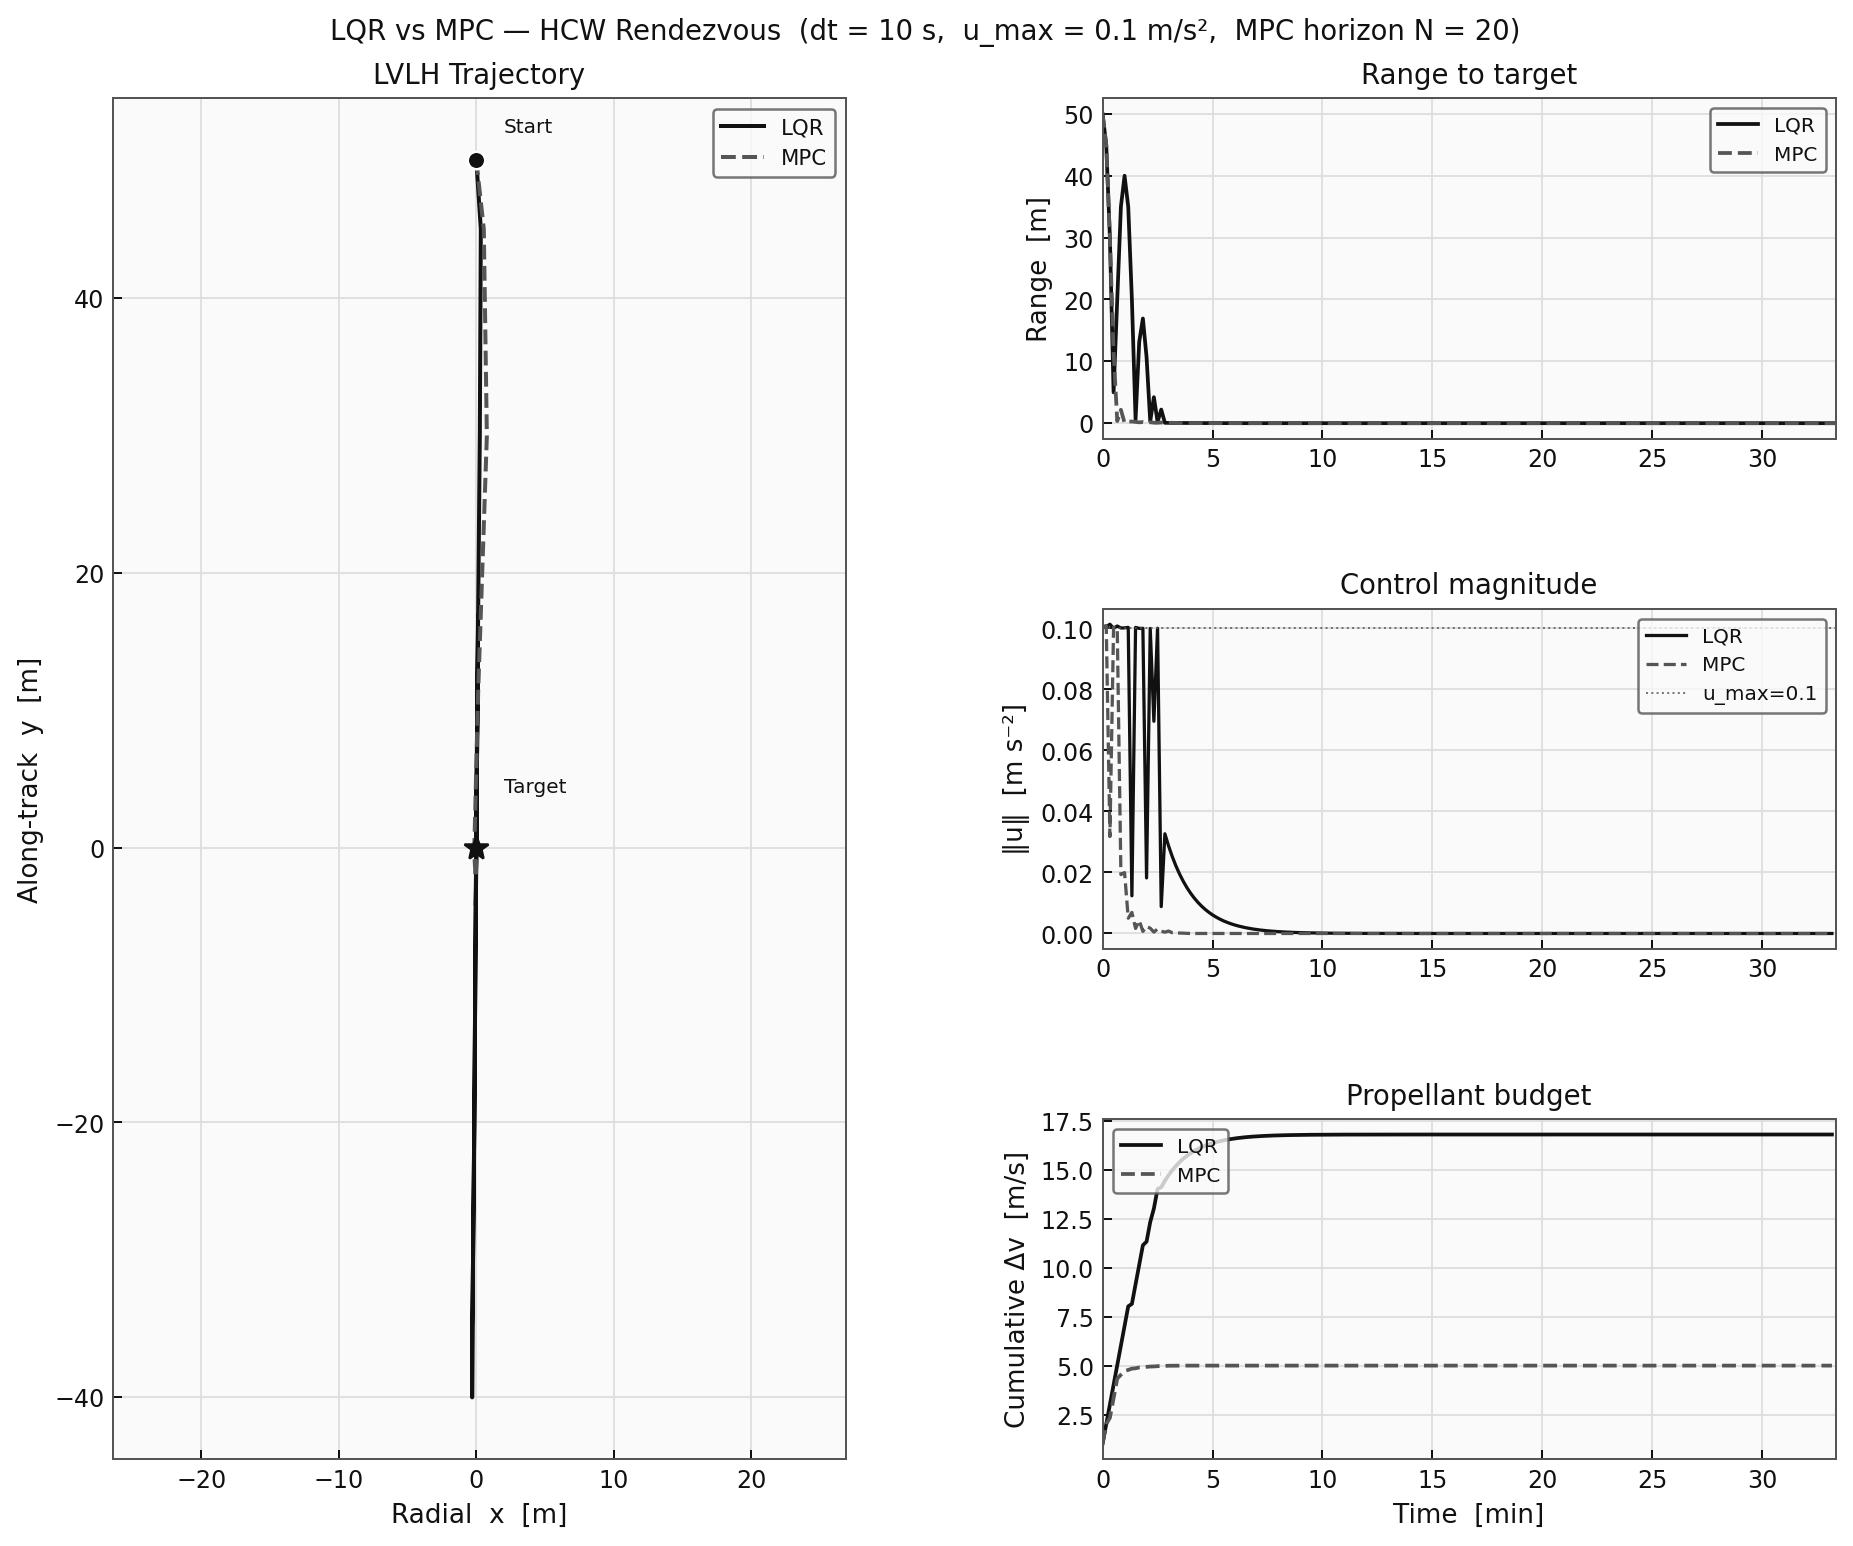
\includegraphics[width=0.86\columnwidth]
    {figures/expE_fig6_lqr_vs_mpc_trajectory.png}
    \caption{LQR and MPC approach trajectories in the LVLH plane.}
    \label{fig:lqr_mpc_traj}
\end{figure}

\subsection{Closed-Loop Performance}
\label{sec:res_closedloop}

The full pipeline was run from a 30~m initial separation with a tumbling
target ($\boldsymbol{\omega}_0 = [0.02,\ 0.05,\ 0.01]$~rad/s).
Table~\ref{tab:closedloop} summarises 12 seeds: all dock, in 2.56~m/s of
$\Delta v$, with no step reaching the thrust limit.

\begin{table}[!tb]
\caption{Closed-loop performance over 12 seeds. Docking is range $<1$~m with
closing speed $<0.05$~m/s.}
\label{tab:closedloop}
\centering
\begin{tabular}{lrr}
\hline
Metric & Mean & Std \\
\hline
Docking step                & 42.7  & 0.6 \\
$\Delta v$ to docking [m/s] & 2.562 & 0.052 \\
Navigation RMSE [m]         & 0.345 & 0.017 \\
Terminal range [m]          & 0.427 & 0.169 \\
Peak closing speed [m/s]    & 1.332 & 0.027 \\
Vision dropout [\%]         & 36.3  & 0.8 \\
Thrust-saturated steps      & 0     & 0 \\
\hline
\end{tabular}
\end{table}

The absence of saturation is a design requirement rather than an
observation: an LQR gain tuned without regard to the actuator limit demands
approximately ninety times $u_{max}$ at 30~m range, saturates on a quarter of
all steps, arrives at 4~m/s and passes through the target before returning ---
a limit cycle rather than a rendezvous. Weighting control so that the
unsaturated demand respects $u_{max}$, and commanding the controller to a
docking-port hold point on the approach axis rather than to the target centre
of mass, reduces the propellant requirement by a factor of sixteen and the
peak closing speed by a factor of three.

\subsection{Measurement Availability as the Limiting Factor}
\label{sec:res_dropout}

The principal finding of the closed-loop study is that the binding constraint
on this architecture is not pose accuracy but \emph{measurement
availability}, and that availability is governed by geometry rather than by
noise.

Availability must be measured against the range the camera is \emph{at}, not
against the range a trial started from. Every trial that closes traverses the
whole range interval, so a trial-level dropout rate averages the far field,
where every keypoint projects inside the frame, with the terminal phase, where
the target overfills the sensor. That rate is accordingly almost constant
across the dispersion:
$34.3\%$, $33.3\%$ and $31.7\%$ for trials beginning in the 10--20~m, 20--30~m
and 30--50~m bands respectively, which says nothing at all.
Table~\ref{tab:dropout} therefore pools the per-step outcome of every step of
every trial in the dispersed campaign of Section~\ref{sec:res_configs} and
bins it by instantaneous range.

\begin{table}[!tb]
\caption{Measurement availability against instantaneous range, pooled over
3887 control steps of 100 dispersed Monte Carlo trials at
$\sigma_{px} = 1.5$~px. A solve is attempted only when at least six keypoints
pass the visibility gate. Intervals are Wilson 95\,\% score intervals on the
per-step availability.}
\label{tab:dropout}
\centering
\begin{tabular}{lrrrr}
\hline
Range [m] & Steps & Mean visible & Availability & 95\,\% CI \\
\hline
10--50   & 1686 & 15.00 & 100.0\% & [99.8,\,100.0] \\
8--10    & 201 & 14.44 & 100.0\% & [98.1,\,100.0] \\
6--8     & 234 & 10.93 & 100.0\% & [98.4,\,100.0] \\
5--6     & 131 &  8.63 &  96.9\% & [92.4,\,98.8] \\
4--5     & 156 &  7.83 &  85.3\% & [78.8,\,90.0] \\
3--4     & 167 &  7.07 &  67.1\% & [59.6,\,73.7] \\
2--3     & 212 &  4.83 &  26.9\% & [21.4,\,33.2] \\
1--2     & 318 &  3.42 &   9.7\% & [7.0,\,13.5] \\
$<1$     & 782 &  2.51 &   1.8\% & [1.1,\,3.0] \\
\hline
\end{tabular}
\end{table}

The profile is a step, not a gradient: availability is statistically
indistinguishable from unity at every range beyond 6~m and falls by a factor
of fifty-five between the 5--6~m and the sub-metre bins.

The mechanism is field-of-view exit, and it is predictable in closed form. A
target of characteristic length $L$ fills a sensor of width $W$ pixels at a
range
\begin{equation}
z_{fill} = \frac{f L}{W},
\label{eq:zfill}
\end{equation}
which for the 8~m Ariane upper stage with $f = 800$~px and $W = 1024$~px gives
$z_{fill} = 6.25$~m. The first bin in Table~\ref{tab:dropout} whose
availability interval excludes unity is 5--6~m, immediately inside that
prediction. Inside $z_{fill}$ the number of keypoints simultaneously within the
image falls below the six required for a minimal RANSAC sample --- the mean
visible count crosses six between the 4--5~m and 3--4~m bins --- and the pose
solution becomes unavailable regardless of detector accuracy.

This has a direct consequence for the noise ablation.
Table~\ref{tab:ablation} sweeps $\sigma_{px}$ over 40 dispersed trials per
level, \emph{paired}: the same seed sequence generates the initial position,
velocity, tumble rate and attitude at every noise level, so the level-to-level
difference is the effect of the parameter and not of a fresh draw of initial
conditions.

\begin{table}[!tb]
\caption{Terminal accuracy and docking success against keypoint noise. 40
dispersed trials per level, paired across levels, full vision--MEKF pipeline.
Terminal range is reported as the median with 5th and 95th percentiles: a
single diverging trial dominates the mean and its standard deviation.
Docking intervals are Wilson 95\,\% score intervals.}
\label{tab:ablation}
\centering
\begin{tabular}{lrrr}
\hline
$\sigma_{px}$ [px] & Terminal range [m] & Docking & 95\,\% CI \\
\hline
0.3 & 0.34 [0.11,\,0.78]  & 100\% & [91,\,100] \\
0.7 & 0.33 [0.14,\,0.82]  & 100\% & [91,\,100] \\
1.0 & 0.32 [0.11,\,0.81]  & 100\% & [91,\,100] \\
1.5 & 0.30 [0.13,\,0.82]  & 100\% & [91,\,100] \\
2.0 & 0.32 [0.09,\,0.73]  &  98\% & [87,\,100] \\
3.0 & 0.34 [0.15,\,8.22]  &  95\% & [83,\,99]  \\
4.0 & 0.51 [0.17,\,12.47] &  85\% & [71,\,93]  \\
\hline
\end{tabular}
\end{table}

The median terminal range is flat from 0.3 to 3.0~px --- it varies by 4~cm
while the noise grows tenfold --- and the degradation appears first in the
\emph{tail}, not in the centre of the distribution. The 95th percentile rises
from 0.73~m at 2~px to 8.22~m at 3~px and 12.47~m at 4~px, and docking success
falls from $100\%$ to $85\%$ over the same interval. The median trial at 4~px
docks as tightly as the median trial at 0.3~px while roughly one trial in
seven diverges completely: the signature of a threshold, not of drift. The
threshold is the point at which the pose solver's success rate inside $z_{fill}$ falls low
enough that the filter coasts on prediction for the whole terminal phase, and
the accumulated dead-reckoning error exceeds the docking corridor before the
range gate is satisfied.

The dispersion also weakens a conclusion that a single-trajectory study would
have supported. Repeating this ablation along one fixed approach trajectory,
varying only the noise realisation, yields a far sharper collapse --- 65\%
success at 4~px with a terminal-range standard deviation above 100~m ---
because every trial then encounters the field-of-view knee at the same
geometry and the same phase of the tumble. Dispersing the initial condition
spreads that encounter, and the honest statement of the effect is the milder
one in Table~\ref{tab:ablation}. We report both because the difference is
itself the argument for dispersing: a Monte Carlo campaign that varies only
the random seed measures the repeatability of one trajectory, not the
robustness of a design.

Two implications follow. First, the useful figure of merit for a monocular
front end in this role is not pose RMSE but the probability of returning a
usable solution, and the two do not degrade together: between 0.3 and 2.0~px
the pose error grows by a factor of seven (Table~\ref{tab:pose_noise}) while
closed-loop performance is unchanged. Second, terminal approach inside
$z_{fill}$ requires a change of sensing modality --- a wider lens, a second
short-range camera, or a close-range keypoint subset chosen to remain in
frame --- and no improvement in the pose solver will substitute for it. The
design margin worth buying is field of view and keypoint redundancy at short
range, not sub-pixel feature localisation.

\begin{figure}[!tb]
    \centering
    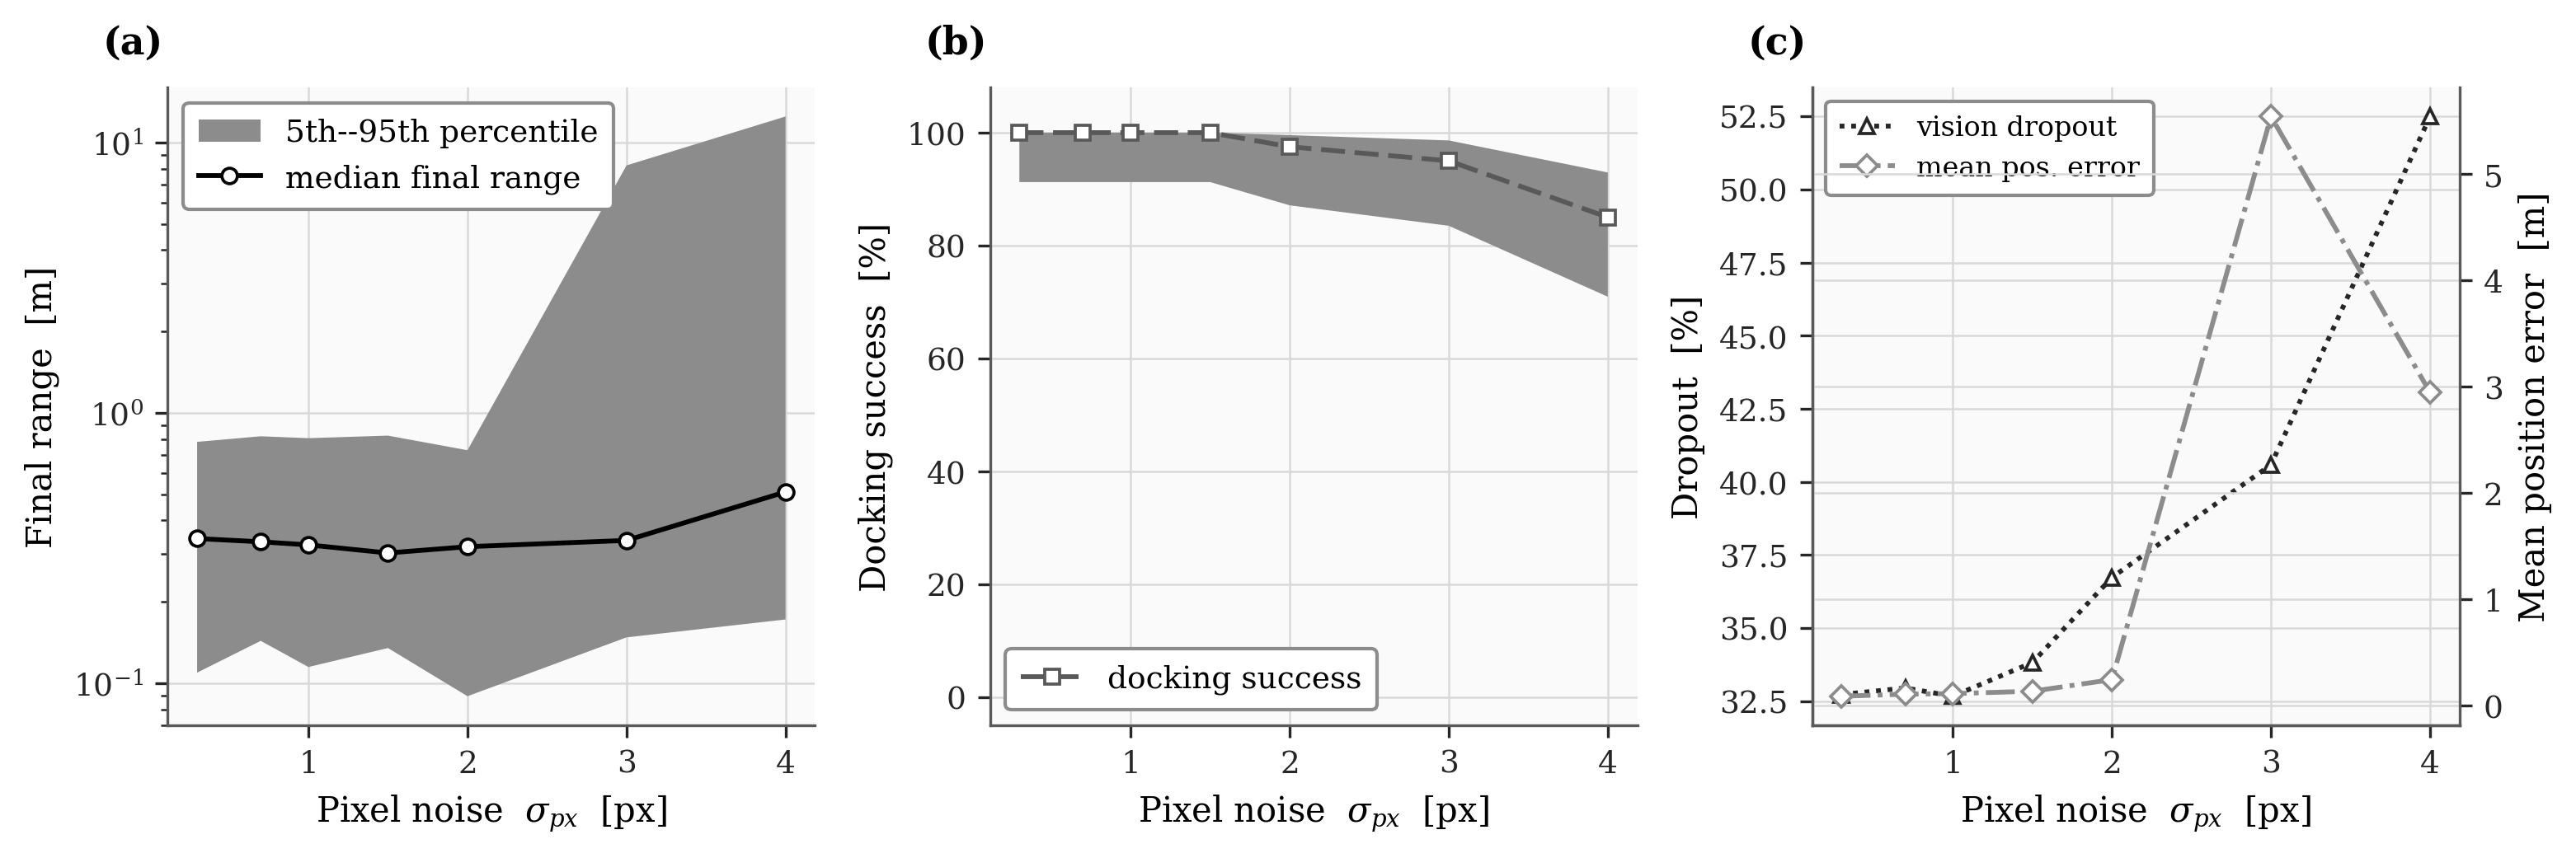
\includegraphics[width=0.86\columnwidth]
    {figures/expF_fig9_ablation_noise.png}
    \caption{Terminal range, docking success and vision dropout against
    keypoint noise, 40 paired dispersed trials per level. The envelope is flat
    to 2~px; the degradation beyond it appears in the tail of the terminal
    range distribution while the median is unchanged.}
    \label{fig:ablation}
\end{figure}

\begin{figure}[!tb]
    \centering
    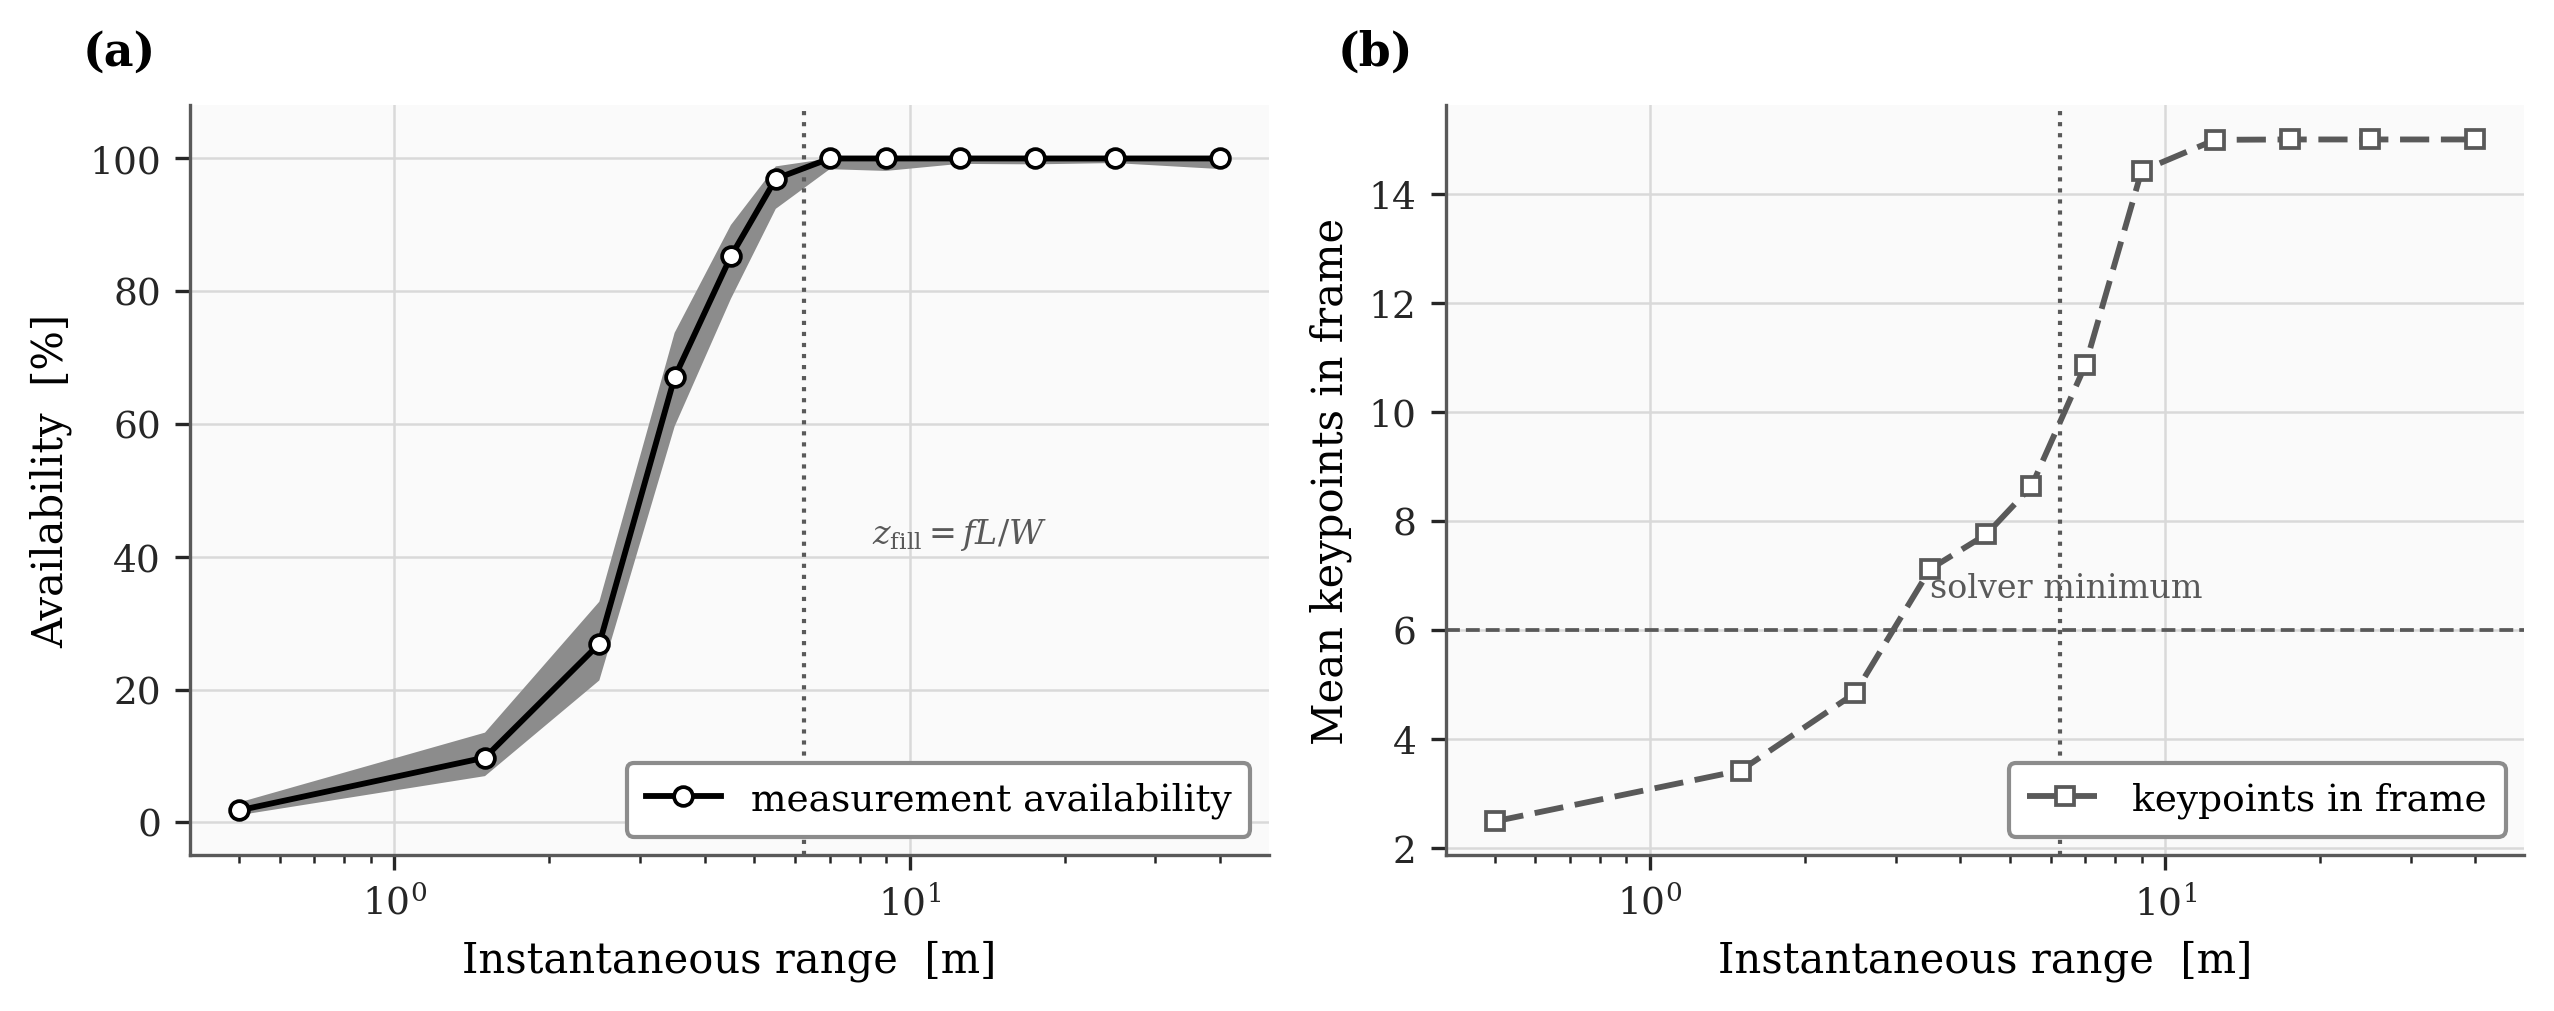
\includegraphics[width=0.86\columnwidth]
    {figures/expF_fig10_availability.png}
    \caption{(a) Per-step measurement availability against instantaneous
    range, pooled over the 100-trial dispersed campaign, with the closed-form
    fill range $z_{fill} = fL/W = 6.25$~m marked. Shading is the Wilson
    95\,\% interval. (b) Mean number of keypoints passing the visibility gate;
    the six-keypoint solver minimum is crossed just inside $z_{fill}$.}
    \label{fig:availability}
\end{figure}

\subsection{Dispersed Monte Carlo Campaign}
\label{sec:res_configs}

The configurations are compared over a dispersed Monte Carlo campaign rather
than over repeated runs of one trajectory. Each trial draws an initial range log-uniformly on $[15, 45]$~m, a bearing uniformly within a
$20^{\circ}$ cone about the radial approach axis, a closing speed uniformly on
$[-0.15, -0.02]$~m/s with a $1\,\mathrm{cm/s}$ transverse component, a tumble
rate uniformly on $[0.005, 0.09]$~rad/s about an isotropically distributed
axis, an initial target attitude uniform on $SO(3)$ by Shoemake's method, and
a navigation initialisation error of $1.5$~m and $2$~cm/s per axis
$(1\sigma)$. Trials are seeded from a single \texttt{SeedSequence}, spawned
per trial and split again into an independent dispersion stream and simulator
stream, so any trial is reproducible in isolation, is independent of the
campaign size and of execution order, and is identical whether the campaign
runs serially or in parallel. The three configurations share that seed
sequence and are therefore compared trial-by-trial on identical initial
conditions.

\begin{table}[!tb]
\caption{Configuration comparison over 100 dispersed trials each, paired
across configurations, $\sigma_{px} = 1.5$~px where applicable. Terminal range
is the median with 5th and 95th percentiles; docking intervals are Wilson
95\,\% score intervals.}
\label{tab:configs}
\centering
\begin{tabular}{lrrr}
\hline
Configuration & Range [m] & $\Delta v$ [m/s] & Docking \\
\hline
Perfect state             & 0.33 & $2.53 \pm 0.80$ & 100\% [96,\,100] \\
Direct measurement + MEKF & 0.54 & $2.65 \pm 0.81$ & 100\% [96,\,100] \\
Full vision + MEKF        & 0.33 & $2.52 \pm 0.80$ & 100\% [96,\,100] \\
\hline
\end{tabular}
\end{table}

The three configurations lie within 5\% of one another in propellant and dock
in every one of the 300 trials. We draw a deliberately narrow conclusion: at
$\sigma_{px} = 1.5$~px the perception chain is \emph{not} the limiting
subsystem, and closed-loop performance is set by the guidance law and the
actuator limit. It would be a mistake to read the full pipeline's marginal
advantage over the direct-measurement baseline as evidence that vision
outperforms a half-metre position sensor: the two configurations have
different measurement error magnitudes, and the comparison is informative only
about which subsystem is binding --- which at this noise level is neither. It
becomes discriminating only above 3~px, where Table~\ref{tab:ablation} shows
the perception chain taking over as the limiting factor.

Two aspects of the campaign design are worth stating explicitly, because both
were defects in an earlier version of this study. First, the perfect-state
configuration has no sensor noise anywhere, so if only the random seed were
varied its trials would be bit-identical and its reported distribution would
be an artefact; dispersing the initial condition gives it a genuine
distribution, and the $\Delta v$ spread of $\pm 0.80$~m/s in
Table~\ref{tab:configs} is the spread induced by the initial condition alone,
which is the correct baseline against which to read the other two rows.
Second, mean $\Delta v$ over all trials is not a propellant budget when some
trials fail, so the campaign reports it conditioned on docking as well; here
the two coincide because every trial docked, but they diverge in the ablation
of Table~\ref{tab:ablation}.
